

\section{Prueba 4}

\subsection{Red de inferencia}
\begin{center}
	\tikzstyle{regla}= [rectangle,draw,black,fill=blue!15]
	\tikzstyle{hecho}= [rectangle,draw,black,fill=black!15]
	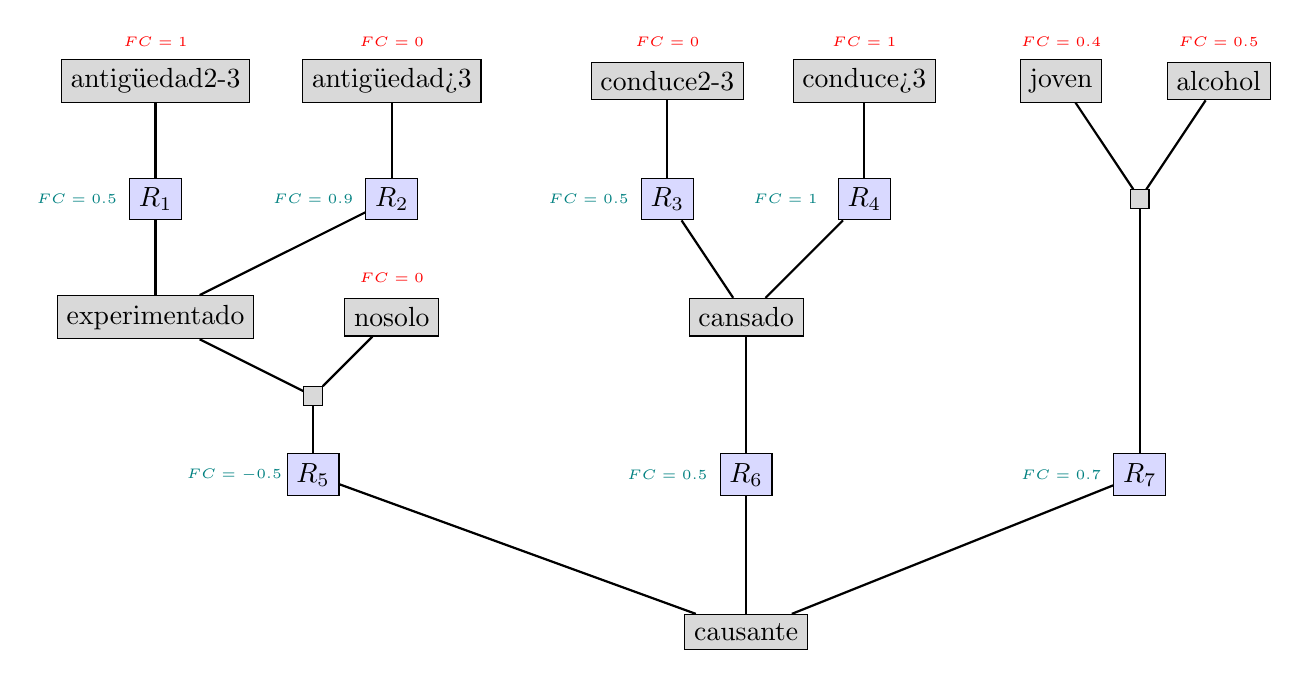
\begin{tikzpicture}
		
		\node (a) at (-3,5) [hecho] {antigüedad2-3};
		\node at (-3,5.5) {\color{red}{\tiny{$FC=1$}}};

		\node (b) at (0,5) [hecho] {antigüedad>3};
		\node at (0,5.5) {\color{red}{\tiny{$FC=0$}}};

		\node (c) at (3.5,5) [hecho] {conduce2-3};
		\node at (3.5,5.5) {\color{red}{\tiny{$FC=0$}}};

		\node (d) at (6,5)[hecho] {conduce>3};
		\node at (6,5.5) {\color{red}{\tiny{$FC=1$}}};

		\node (e) at (-3,2)[hecho] {experimentado};
		
		\node (f) at (4.5,2)[hecho] {cansado};

		\node (g) at (8.5,5)[hecho] {joven};
		\node at (8.5,5.5) {\color{red}{\tiny{$FC=0.4$}}};

		\node (h) at (10.5,5)[hecho] {alcohol};
		\node at (10.5,5.5) {\color{red}{\tiny{$FC=0.5$}}};

		\node (i) at (0,2)[hecho] {nosolo};
		\node at (0,2.5) {\color{red}{\tiny{$FC=0$}}};

		\node (j) at (4.5,-2)[hecho] {causante};

		\node (e/i) at (-1,1)[hecho] {};
		\node (g/h) at (9.5,3.5)[hecho] {};

		\node (r1) at (-3,3.5) [regla] {$R_{1}$};
		\node at (-4,3.5) {\color{teal}{\tiny{$FC=0.5$}}};
		\node (r2) at (0,3.5) [regla] {$R_{2}$};
		\node at (-1,3.5) {\color{teal}{\tiny{$FC=0.9$}}};
		\node (r3) at (3.5,3.5) [regla] {$R_{3}$};
		\node at (2.5,3.5) {\color{teal}{\tiny{$FC=0.5$}}};
		\node (r4) at (6,3.5) [regla] {$R_{4}$};
		\node at (5,3.5) {\color{teal}{\tiny{$FC=1$}}};
		\node (r5) at (-1,0) [regla] {$R_{5}$};
		\node at (-2,0) {\color{teal}{\tiny{$FC=-0.5$}}};
		\node (r6) at (4.5,0) [regla] {$R_{6}$};
		\node at (3.5,0) {\color{teal}{\tiny{$FC=0.5$}}};
		\node (r7) at (9.5,0) [regla] {$R_{7}$};
		\node at (8.5,0) {\color{teal}{\tiny{$FC=0.7$}}};

		\path[black,thick] (a) edge[] node {} (r1);
		\path[black,thick] (r1) edge[] node {} (e);
		\path[black,thick] (b) edge[] node {} (r2);
		\path[black,thick] (r2) edge[] node {} (e);
		\path[black,thick] (e) edge[] node {} (e/i);
		\path[black,thick] (i) edge[] node {} (e/i);
		\path[black,thick] (e/i) edge[] node {} (r5);
		\path[black,thick] (r5) edge[] node {} (j);
	
	
		\path[black,thick] (c) edge[] node {} (r3);
		\path[black,thick] (r3) edge[] node {} (f);
		\path[black,thick] (d) edge[] node {} (r4);
		\path[black,thick] (r4) edge[] node {} (f);
		\path[black,thick] (f) edge[] node {} (r6);
		\path[black,thick] (r6) edge[] node {} (j);

		\path[black,thick] (g) edge[] node {} (g/h);
		\path[black,thick] (h) edge[] node {} (g/h);
		\path[black,thick] (g/h) edge[] node {} (r7);
		\path[black,thick] (r7) edge[] node {} (j);

	\end{tikzpicture}
\end{center}
\par Esta red de inferencia se debe interpretar de arriba a abajo.
Los rectángulos azules son las reglas, los grises que están ligados por encima 
de ellas son sus antecedentes, si estos antecedentes convergen en un cuadrado 
quiere decir que es la conjunción de esos literales, en caso contrario son disyunciones
o simplemente un literal. Los rectángulos grises que cuelgan de las reglas 
son sus consecuentes respectivamente. Además, incluyo los factores de certeza propocionados por
la Base de hechos y la Base de Conocimiento iniciales.

\subsection{Proceso de inferencia}
\begin{listing}[language=Pascal]
(Razonamiento dirigido por Metas)
Objetivo: causante
Proceso de Inferencia: 
  ###########################
  # Llamada (1) a verificar #
  ###########################
	Verificar(causante,{alcohol,antiguedad2-3,antiguedad>3,
	conduce2-3,conduce>3,joven,nosolo}) // Recursion 
	Conjunto Conflicto={R5,R6,R7} // causante es consecuente de estas reglas
	R={R5} // Seleccionar regla R5
	Eliminar R5 ---> Conjunto Conflicto={R6,R7}
	NuevasMetas={experimentado,nosolo} // Antecedentes de R5; Verificado = true
	Meta=experimentado // Seleccionar experimentado de NuevasMetas
	NuevasMetas={nosolo} // Eliminar experimentado de NuevasMetas
  ###########################
  # Llamada (2) a verificar #
  ###########################
	Verificar(experimentado,{alcohol,antiguedad2-3,
	antiguedad>3,conduce2-3,conduce>3,joven,nosolo})    // Recursion 
	Conjunto Conflicto={R1,R2} // experimentado es consecuente de estas reglas
	R={R1} // Seleccionar regla R1
	Eliminar R1 ---> Conjunto Conflicto={R2,}
	NuevasMetas={antiguedad2-3} // Antecedentes de R1; Verificado = true
	Meta=antiguedad2-3 // Seleccionar antiguedad2-3 de NuevasMetas
	NuevasMetas={} // Eliminar antiguedad2-3 de NuevasMetas
  ###########################
  # Llamada (3) a verificar #
  ###########################
	Verificar(antiguedad2-3,{alcohol,antiguedad2-3,
	antiguedad>3,conduce2-3,conduce>3,joven,nosolo})   ---> true // Recursion: antiguedad2-3 en BH
	BH={alcohol,antiguedad2-3,antiguedad>3,conduce2-3, 
	conduce>3,joven,nosolo}
	(CASO 3): Combinacion de la evidencia con la regla R1
	 FC(experimentado{R1})=0.5*max(0,FC(antiguedad2-3))=0.5
	Conjunto Conflicto={R2} // experimentado es consecuente de estas reglas
	R={R2} // Seleccionar regla R2
	Eliminar R2 ---> Conjunto Conflicto={}
	NuevasMetas={antiguedad>3,} // Antecedentes de R2; Verificado = true
	Meta=antiguedad>3 // Seleccionar antiguedad>3 de NuevasMetas
	NuevasMetas={} // Eliminar antiguedad>3 de NuevasMetas
  ###########################
  # Llamada (4) a verificar #
  ###########################
	Verificar(antiguedad>3,{alcohol,antiguedad2-3,
	antiguedad>3,conduce2-3,conduce>3,joven,nosolo}) ---> true // Recursion: antiguedad>3 en BH
	BH={alcohol,antiguedad2-3,antiguedad>3,conduce2-3,
	conduce>3,joven,nosolo}
	(CASO 3): Combinacion de la evidencia con la regla R2
	 FC(experimentado{R2})=0.9*max(0,FC(antiguedad>3))=0
	(CASO 2): Combinacion de las reglas R1 y R2
	 FC(experimentado)=FC(experimentado{R1}) + FC(experimentado{R2})*(1-FC(experimentado{R1}))=0.5
	BH={alcohol,antiguedad2-3,antiguedad>3,conduce2-3,
	conduce>3,experimentado,joven,nosolo} // Insertar experimentado a la Base de Hechos
	Meta=nosolo // Seleccionar nosolo de NuevasMetas
	NuevasMetas={} // Eliminar nosolo de NuevasMetas
  ###########################
  # Llamada (5) a verificar #
  ###########################
	Verificar(nosolo,{alcohol,antiguedad2-3,antiguedad>3,
	conduce2-3,conduce>3,experimentado,joven,nosolo}) ---> true // Recursion: nosolo en BH
	BH={alcohol,antiguedad2-3,antiguedad>3,conduce2-3,
	conduce>3,experimentado,joven,nosolo}
	(CASO 1): Combinacion de antecedentes de R5
	 FC(experimentado y nosolo)=min(FC(experimentado),FC(nosolo))=0
	(CASO 3): Combinacion de la evidencia con la regla R5
	 FC(causante{R5})=-0.5*max(0,FC(experimentado y nosolo))=-0
	Conjunto Conflicto={R6,R7} // causante es consecuente de estas reglas
	R={R6} // Seleccionar regla R6
	Eliminar R6 ---> Conjunto Conflicto={R7}
	NuevasMetas={cansado} // Antecedentes de R6; Verificado = true
	Meta=cansado // Seleccionar cansado de NuevasMetas
	NuevasMetas={} // Eliminar cansado de NuevasMetas
  ###########################
  # Llamada (6) a verificar #
  ###########################
	Verificar(cansado,{alcohol,antiguedad2-3,antiguedad>3,
	conduce2-3,conduce>3,experimentado,joven,nosolo})   // Recursion 
	Conjunto Conflicto={R3,R4} // cansado es consecuente de estas reglas
	R={R3} // Seleccionar regla R3
	Eliminar R3 ---> Conjunto Conflicto={R4}
	NuevasMetas={conduce2-3} // Antecedentes de R3; Verificado = true
	Meta=conduce2-3 // Seleccionar conduce2-3 de NuevasMetas
	NuevasMetas={} // Eliminar conduce2-3 de NuevasMetas
  ###########################
  # Llamada (7) a verificar #
  ###########################
	Verificar(conduce2-3,{alcohol,antiguedad2-3,
	antiguedad>3,conduce2-3,conduce>3,experimentado,joven,
	nosolo}) ---> true // Recursion: conduce2-3 en BH
	BH={alcohol,antiguedad2-3,antiguedad>3,conduce2-3,
	conduce>3,experimentado,joven,nosolo}
	(CASO 1): Combinacion de antecedentes de R3
	 FC(conduce2-3)=min(FC(conduce2-3))=0
	(CASO 3): Combinacion de la evidencia con la regla R3
	 FC(cansado{R3})=0.5*max(0,FC(conduce2-3))=0
	Conjunto Conflicto={R4} // cansado es consecuente de estas reglas
	R={R4} // Seleccionar regla R4
	Eliminar R4 ---> Conjunto Conflicto={}
	NuevasMetas={conduce>3} // Antecedentes de R4; Verificado = true
	Meta=conduce>3 // Seleccionar conduce>3 de NuevasMetas
	NuevasMetas={} // Eliminar conduce>3 de NuevasMetas
  ###########################
  # Llamada (8) a verificar #
  ###########################
  	Verificar(conduce>3,{alcohol,antiguedad2-3,antiguedad>3,
	conduce2-3,conduce>3,experimentado,joven,nosolo}) ---> true // Recursion: conduce>3 en BH
	BH={alcohol,antiguedad2-3,antiguedad>3,conduce2-3,
	conduce>3,experimentado,joven,nosolo}
	(CASO 1): Combinacion de antecedentes de R4
	 FC(conduce>3)=min(FC(conduce>3))=1
	(CASO 3): Combinacion de la evidencia con la regla R4
	 FC(cansado{R4})=1*max(0,FC(conduce>3))=1
	(CASO 2): Combinacion de las reglas R3 y R4
	 FC(cansado)=FC(cansado{R3}) + FC(cansado{R4})*(1-FC(cansado{R3}))=1
	BH={alcohol,antiguedad2-3,antiguedad>3,cansado,
	conduce2-3,conduce>3,experimentado,joven,nosolo} // Insertar cansado a la Base de Hechos
	(CASO 3): Combinacion de la evidencia con la regla R6
	 FC(causante{R6})=0.5*max(0,FC(cansado))=0.5
	Conjunto Conflicto={R7,} // causante es consecuente de estas reglas
	R={R7} // Seleccionar regla R7
	Eliminar R7 ---> Conjunto Conflicto={}
	NuevasMetas={alcohol,joven} // Antecedentes de R7; Verificado = true
	Meta=alcohol // Seleccionar alcohol de NuevasMetas
	NuevasMetas={joven} // Eliminar alcohol de NuevasMetas
  ###########################
  # Llamada (9) a verificar #
  ###########################
	Verificar(alcohol,{alcohol,antiguedad2-3,antiguedad>3,
	cansado,conduce2-3,conduce>3,experimentado,joven,
	nosolo}) ---> true // Recursion: alcohol en BH
	BH={alcohol,antiguedad2-3,antiguedad>3,cansado,
	conduce2-3,conduce>3,experimentado,joven,nosolo}
	Meta=joven // Seleccionar joven de NuevasMetas
	NuevasMetas={} // Eliminar joven de NuevasMetas
  ###########################
  # Llamada (10) a verificar #
  ###########################
	Verificar(joven,{alcohol,antiguedad2-3,antiguedad>3,
	cansado,conduce2-3,conduce>3,experimentado,joven,
	nosolo}) ---> true // Recursion: joven en BH
	BH={alcohol,antiguedad2-3,antiguedad>3,cansado,
	conduce2-3,conduce>3,experimentado,joven,nosolo}
	(CASO 1): Combinacion de antecedentes de R7
	 FC(joven y alcohol)=min(FC(alcohol),FC(joven))=0.4
	(CASO 3): Combinacion de la evidencia con la regla R7
	 FC(causante{R7})=0.7*max(0,FC(joven y alcohol))=0.28
	(CASO 2): Combinacion de las reglas R5 y R6
	 FC(causante)=FC(causante{R5}) + FC(causante{R6})*(1-FC(causante{R5}))=0.5
	(CASO 2): Combinacion de las reglas R3 y R7
	 FC(causante)=FC(causante{R3}) + FC(causante{R7})*(1-FC(causante{R3}))=0.64
	BH={alcohol,antiguedad2-3,antiguedad>3,cansado,
	causante,conduce2-3,conduce>3,experimentado,joven,
	nosolo} // Insertar causante a la Base de Hechos
Return TRUE
\end{listing}
\subsection{Objetivo obtenido por SBR-FC}
\begin{center}
\par -------------------- Hecho (causante) ---------------------
\par Hecho (nomHecho): causante
\par Hecho (facCerBH): 0.64
\par ------------------------------------------------------------
\end{center}
\subsection{Cuestión}
\begin{ejer}
	\textbf{Prueba 4.} Un \texttt{conductor} de 32 años (entendemos que es joven con grado 0.4), 
	con 2-3 años de antigüedad, ha conducido durante más de 3 horas, viajaba solo y 
	había bebido algo de alcohol (entendemos que su factor de certeza es de 0.5). \\
	¿Cuál será el grado de certeza de que este conductor ha sido causante del accidente?
\end{ejer}
\par Solución: El grado de certeza es 0.64.